\chapter{Bifurcaciones}
Ya hemos estudiado y clasificado el comportamiento cualitativo global de sistemas lineales y local en sistemas no lineales, cerca de puntos críticos. En general, en presencia de equilibrios hiperbólicos esta clasificación está completa. En caso contrario es necesario hacer un análisis propio del sistema.

Consideramos ahora sistemas que dependen de un parámetro $\lambda$, de la forma

\begin{equation} \label{eq:sistemabifurcacion}
	\dot{x} = f(x, \lambda).
\end{equation}

Podría ocurrir que al variar el parámetro $\lambda$ los puntos críticos del sistema \ref{eq:sistemabifurcacion} aparezcan o desaparezcan, se estabilicen o desestabilicen o cambien de tipo y, en consecuencia, el comportamiento cualitativo del sistema (su diagrama de fase) cambie notablemente.

Ya en el ejemplo \ref{ex:nolinealnohiperbolico}, vimos un sistema en el que siempre aparece el punto crítico $x = 0$ pero éste cambia de estabilidad según el parámetro $\mu$ sea positivo, negativo o nulo.

Las otras posibilidades mencionadas también pueden ocurrir en otros sistemas planos.

\begin{definition} \label{def:bifurcacion}
Sea $f$ una función que depende continuamente tanto de $x$ como del parámetro $\lambda$. Si un cambio suave en $\lambda$ produce un cambio cualitativo o topológico en el comportamiento del sistema plano $\dot{x} = f(x,\lambda)$, se dice que ha ocurrido una \emph{bifurcación}.
\end{definition}

Las bifurcaciones pueden clasificarse como locales o globales:
\begin{itemize}
	\item Una bifurcación local ocurre cuando el cambio en el parámetro causa un cambio en la estabilidad de un punto de equilibrio.

	Es claro, entonces, que bifurcaciones locales se presentan cuando el sistema linealizado en vecindad de un punto crítico tiene valor propio con parte real que pasa por $0$.
	Esto es, una bifurcación local ocurre en $(x_0, \lambda_0)$ siempre que $Df(x_0, \lambda_0)$ tenga un valor propio con parte real nula.

	Las bifurcaciones locales pueden determinarse a través del estudio de la estabilidad del sistema.

	\item En contraste, las bifurcaciones globales no dependen de la estabilidad local pues se refieren a cambios cualitativos en el comportamiento dentro de conjuntos invariantes más grandes como lo son ciclos límite o trayectorias que se extienden una distancia grande.
\end{itemize}

La aparición de algunas de estas bifurcaciones (en particular las relacionadas con ciclos límite) requieren que el sistema tenga, cuando menos, dos dimensiones. En particular, la existencia de ciclos límite es el teorema de Poincaré-Bendixson (ver teorema \ref{teo:poincarebendixson}) así que este tipo de bifurcaciones ocurren únicamente desde sistemas planos en adelante.

\section{Bifurcaciones esencialmente unidimensionales en sistemas 2-dimensionales}

Consideramos a continuación algunas bifurcaciones que aparecen también en sistemas dinámicos 1-dimensionales.

\subsection{Bifurcación silla-nodo} \label{sec:bifurcacionsillanodo}
Ocurre cuando dos puntos críticos colisionan a medida que el parámetro $\lambda$ cambia y se anulan el uno al otro.

El ejemplo prototípico de una bifurcación silla-nodo es el siguiente.

\begin{example}
$$ 
	\dot{x_1} = \lambda - x_1^2 \hspace{0.5in} \dot{x_2} = -x_2.
$$

Los puntos críticos del sistema son $(\sqrt{\lambda}, 0)$ y $(-\sqrt{\lambda}, 0).$

La matriz jacobiana $Df$ es

$$
Df(\pm \sqrt{\lambda}, 0) = \left( \begin{array}{ll}
	\mp 2 \sqrt{\lambda} & 0 \\
	0 & -1
\end{array} \right),
$$

que tiene valores propios $-1$ y $\mp 2\sqrt{\lambda}$.

\begin{itemize}
	\item Si $\lambda > 0$ el punto crítico $(\sqrt{\lambda}, 0)$ es un nodo asintóticamente estable y $(-\sqrt{\lambda}, 0)$ es un punto de silla inestable.
	\item Mientras $\lambda$ decrece los puntos se acercan uno al otro y en $\lambda = 0$ el sistema tiene un único punto crítico $(0,0)$.
	\item Cuando $\lambda < 0$ no hay puntos críticos.
\end{itemize}

\begin{figure}[ht] \centering
    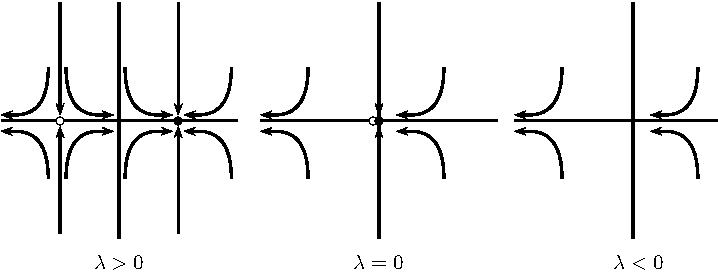
\includegraphics[scale=1.0]{figures/bifurcations-saddlenode.pdf}
    \caption{Bifurcación de silla-nodo.}
\end{figure}

Notamos que aún siendo este un sistema plano, el cambio de dinámica ocurre exclusivamente en el eje $x_1$.
\end{example}

Por supuesto bifurcaciones de este tipo aparecen en sistemas con una forma más general, como en el siguiente teorema.

\begin{theorem}Consideremos el sistema

$$ \dot{x_1} = F_1(x_1, x_2, \lambda) \hspace{0.5in} \dot{x_2} = -x_2 + F_2(x_1, x_2, \lambda). $$

con $F=(F_1,F_2)$ al menos de clase $C^1$ que satisface que $F(x,0) = f(x)$ con $f(0) = 0$ y $Df(0) = 0$.

Si
$$
	\dfrac{\partial F_1}{\partial \lambda}(0,0,0) \neq 0 \hspace{0.5in}
	\dfrac{\partial^2 F_1}{\partial x_1^2}(0,0,0) \neq 0	
$$
entonces existe una bifurcación de silla-nodo en $\lambda = 0$.
Cuando $\lambda \dfrac{\partial F_1}{\partial \lambda} \dfrac{\partial^2 F_1}{\partial x_1^2} < 0$ hay dos puntos de equilibrio hiperbólicos (una silla y el otro un nodo asintóticamente estable) y no hay equilibrios cuando $\lambda \dfrac{\partial F_1}{\partial \lambda} \dfrac{\partial^2 F_1}{\partial x_1^2} > 0$.
\begin{proof}
Ver \cite[p.~316]{dynandbif}.
\end{proof}
\end{theorem}


\subsection{Bifurcación transcrítica}

A diferencia de la bifurcación silla-nodo, en una bifurcación transcrítica un punto crítico existe para todo valor del parámetro $\lambda$ pero intercambian su estabilidad con otro punto crítico luego de la ``colisión'' entre ellos.

\begin{example} \label{ex:transcriticbifurcation}
$$ 
	\dot{x_1} = \lambda x_1 - x_1^2 \hspace{0.5in} \dot{x_2} = -x_2.
$$

Los puntos críticos son $u = (0, 0)$ y $v = (\lambda, 0)$.
La matriz jacobiana de $f$ es

$$ Df(x_1,x_2) = \left( \begin{array}{ll}
	\lambda - 2x_1 & 0 \\
	0 & -1
\end{array} \right). $$

\begin{itemize}
	\item Si $\lambda > 0$ entonces $(0,0)$ es un punto de silla y $(\lambda, 0)$ es un nodo asintóticamente estable.
	\item Cuando $\lambda = 0$ los nodos colisionan en uno solo: $(0,0)$ que es semiestable.
	\item Cuando $\lambda < 0$ la estabilidad se intercambia: $(0,0)$ es un nodo asintóticamente estable y $(\lambda, 0)$ un punto de silla.
\end{itemize}

\begin{figure}[!ht] \centering
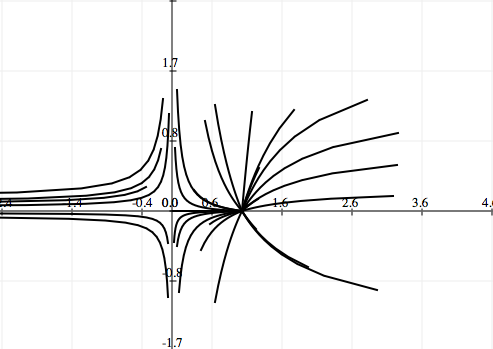
\includegraphics[scale=0.45]{figures/transcriticbifurcation-before.png}
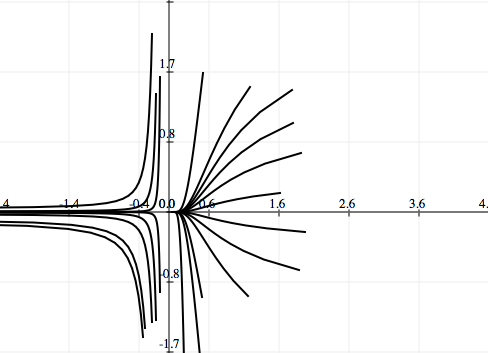
\includegraphics[scale=0.45]{figures/transcriticbifurcation-during.png} \\
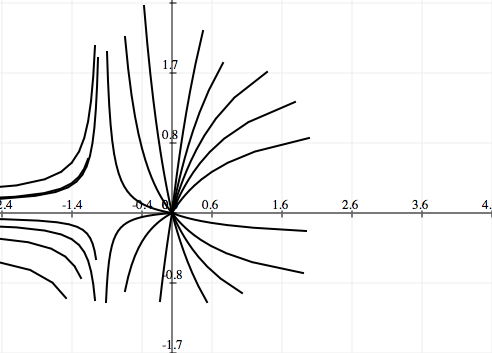
\includegraphics[scale=0.45]{figures/transcriticbifurcation-after.png}
\caption{$\clubsuit$ Diagrama de fase del sistema del ejemplo \ref{ex:transcriticbifurcation} antes, durante y después de una bifurcación transcrítica.}
\end{figure}
\end{example}

\newpage % forzar la figura de transcritica a estar en la misma pagina

\subsection{Bifurcación \textit{pitchfork}}

Ocurre en sistemas dinámicos con simetría. En este tipo de bifurcación el número de equilibrios pasa de 1 a 3 cuando se pasa por el valor de bifurcación del parámetro $\lambda$ y la estabilidad del equilibrio original cambia.

Cuando los otros dos equilibrios que aparecen son estables la bifurcación se dice \emph{supercrítica} y se llama \emph{subcrítica} cuando son inestables.

\begin{example}[Bifurcación \textit{pitchfork} supercrítica]
Considérese el sistema
$$ 
	\dot{x_1} = \lambda x_1 - x_1^3 \hspace{0.5in} \dot{x_2} = -x_2.
$$

El punto crítico $(0,0)$ aparece siempre. Los otros dos posibles puntos críticos son $(\pm \sqrt{\lambda}, 0)$.
La matriz jacobiana de $f$ es

$$
	Df(x_1,x_2) = \left( \begin{array}{ll}
		\lambda - 3x_1^2 & 0 \\
		0 & -1
	\end{array} \right).
$$

\begin{itemize}
	\item Para $\lambda < 0$ el único punto crítico es el origen $(0,0)$ y $Df(0,0)$ tiene valores propios $\lambda < 0$ y $-1$, así que es un nodo asintóticamente estable.
	\item Cuando $\lambda > 0$ el origen $(0,0)$ pierde su estabilidad y aparecen dos nuevos puntos críticos ubicados simétricamente sobre el eje $x_1$. A saber, $(\sqrt{\lambda}, 0)$ y $(-\sqrt{\lambda}, 0)$. 

Como en ambos puntos $Df$ tiene valores propios $-2\lambda$ y $-1$, estos puntos críticos son estables.
\end{itemize}

\begin{figure}[ht] \centering
    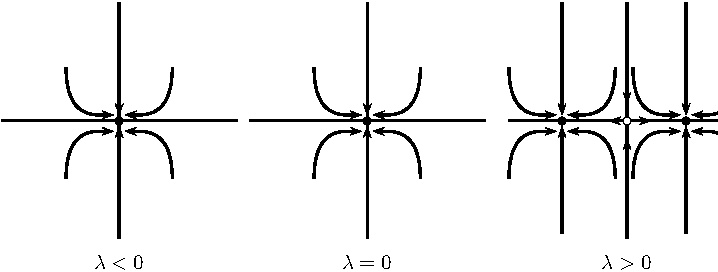
\includegraphics[scale=1.0]{figures/bifurcations-pitchforksupercritical.pdf} 
    \caption{Bifurcación \textit{pitchfork} supercrítica.}
\end{figure}

\end{example}

\begin{example}[Bifurcación \textit{pitchfork} subcrítica]
Consideramos una pequeña modificación del sistema del ejemplo anterior:

$$ 
	\dot{x_1} = \lambda x_1 + x_1^3 \hspace{0.5in} \dot{x_2} = -x_2.
$$

Ahora el punto crítico $(0,0)$ aparece siempre y, posiblemente, los otros dos puntos críticos $(\pm \sqrt{-\lambda}, 0)$.

\begin{itemize}
	\item Cuando $\lambda < 0$ hay tres puntos críticos: $(0,0)$ y $(\pm \sqrt{-\lambda}, 0)$. El origen es estable y los otro dos puntos críticos son inestables.
	\item A medida que $\lambda \to 0$, los tres puntos críticos se acercan hasta que ``colisionan'' y para $\lambda > 0$ el único punto crítico es el origen $(0,0)$ con su estabilidad cambiada: ahora es inestable.
\end{itemize}

% TODO: imagen

\end{example}

Como para las bifurcaciones silla-nodo tenemos un criterio para la aparición de bifurcaciones \textit{pitchfork} en sistemas con formas más complicadas que las de los ejemplos previos.

\begin{theorem}
Considérese el sistema plano $\dot{x} = f(x, \lambda) = f(x_1, x_2, \lambda)$ con $f$ una función suficientemente suave en los tres argumentos. Si $-f(x, \lambda) = f(-x, \lambda)$ y se satisfacen las siguientes condiciones en un $\lambda_0$:

$$
	\dfrac{\partial f}{\partial x_1}(0, \lambda_0) = 0, \dfrac{\partial^2 f}{\partial x_1^2}(0, \lambda_0) = 0, 
	\dfrac{\partial^3 f}{\partial x_1^3}(0, \lambda_0) \neq 0, 
$$

y

$$
	\dfrac{\partial f}{\partial \lambda}(0, \lambda_0) = 0, \dfrac{\partial^2 f}{\partial \lambda x_1}(0, \lambda_0) \neq 0.
$$

Entonces el sistema presenta una bifurcación \textit{pitchfork} cuando $\lambda$ pasa a través de $\lambda_0$ en el origen.
La bifurcación es supercrítica si $\dfrac{\partial^3 f}{\partial x_1^3}(0,\lambda_0) > 0$ y subcrítica si $\dfrac{\partial^3 f}{\partial x_1^3}(0,\lambda_0) < 0$.
\begin{proof}
Ver \cite{strogatz,swiggins}.
\end{proof}
\end{theorem}

\section{Bifurcaciones que requieren al menos dos dimensiones para ocurrir}

Supongamos que un sistema plano $\dot{x} = f(x, \lambda)$ que depende de un parámetro $\lambda$ tiene un punto fijo en $\bar{x}$ y que la matriz jacobiana $Df(\bar{x}, \lambda)$ tiene valores propios $\mu_1, \mu_2$.

Supongamos además que $\bar{x}$ es estable. Es decir, $\Re(\mu_{1,2}) < 0$, de manera que los eigenvalores se encuentran del lado izquierdo del plano complejo.
La única manera en la que la estabilidad del punto crítico cambie es cuando estos eigenvalores (al variar el parámetro $\lambda$) crucen el eje imaginario.

\begin{figure}[ht] \centering
    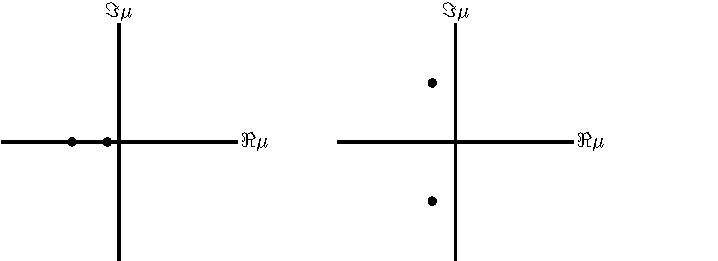
\includegraphics[scale=1.0]{figures/bifurcations-2dimensional.pdf}
\end{figure}

En particular, si los eigenvalores tienen parte imaginaria nula $\Im(\mu_{1,2}) = 0$ entonces se encuentran sobre el eje real y la única posibilidad es que cambien de signo, lo que corresponde a una de las bifurcaciones estudiadas en la sección anterior.
De ahí que se dijera que son esencialmente unidimensionales.

Si en cambio los eigenvalores no tienen parte imaginaria nula, lo que únicamente ocurre en sistemas dinámicos de al menos 2 dimensiones, el comportamiento puede ser más amplio y, debido a la parte imaginaria, involucrar la aparición o desaparición de órbitas periódicas (u órbitas límite).

Uno de estas bifurcaciones más comunes es la de Poincaré-Andronov-Hopf, que estudiamos a continuación.

\subsection{Bifurcación de Poincaré-Andronov-Hopf}

Queremos ver qué sucede en vecindad de un equilibrio no hiperbólico con valores propios imaginarios puros. Del teorema de la función implícita se sigue que bajo perturbaciones pequeñas de $\lambda$ del flujo $f$, el punto crítico no desaparece y no se crean nuevos puntos críticos.

Sin embargo, nada está dicho acerca de la aparición o desaparición de órbitas límite. En la bifurcación de Poincaré-Andronov-Hopf una órbita límite aparece ``de la nada'' mientras el parámetro $\lambda$ varía.

El siguiente teorema establece algunas condiciones para que lo anterior ocurra.

\begin{theorem}[Poincaré-Andronov-Hopf] \label{teo:poincare-andronov-hopf} Sea $\dot{x} = f(x,\lambda) = A(\lambda)x + F(x,\lambda)$ un sistema dinámico de clase al menos $C^3$ con $F(0,\lambda) = 0$ y $\dfrac{\partial F}{\partial x_1}(0, \lambda) = \dfrac{\partial F}{\partial x_2}(0, \lambda) = 0$ para todo $|\lambda|$ suficientemente pequeño. Supóngase que la parte lineal $A(\lambda)$ tiene, en el origen, valores propios $\alpha(\lambda) + i\beta(\lambda)$ con $\alpha(0) = 0$ y $\beta(0) \neq 0$.
Además, supóngase que estos valores propios cruzan el eje imaginario con velocidad no cero, es decir, $\dfrac{d\alpha}{d\lambda}(0) \neq 0$.

Entonces en cualquier vecindad $U \subseteq \R^2$ del origen $(0,0)$ y dado cualquier $\lambda_0 > 0$ existe un $\bar{\lambda}$ con $|\bar{\lambda}| < \lambda_0$ tal que la ecuación diferencial $\dot{x} = A(\bar{\lambda}) + F(x, \bar{\lambda})$ tiene una orbita periódica no trivial en $U$.
\begin{proof}
Ver \cite[p.~344]{dynandbif}.
\end{proof}
\end{theorem}

\begin{example} \label{ex:vanderpol-hopf}
Regresamos al oscilador de Van der Pol, introducido en el ejemplo \ref{ex:vanderpol}:
$$
	\dot{x_1} = x_2, \hspace{0.5in} \dot{x_2} = -x_1 + 2\lambda x_2 - x_1^2 x_2 = (2\lambda - x_1^2)x_2 - x_1.
$$

Comprobemos que el oscilador de Van der Pol presenta una bifurcación de Hopf cuando $\lambda$ pasa a través de $0$.

En forma matricial:

$$
	\begin{pmatrix}\dot{x_1} \\ \dot{x_2}\end{pmatrix} =	\begin{pmatrix}0 & 1 \\ -1 & 2\lambda \end{pmatrix} \begin{pmatrix}x_1 \\ x_2 \end{pmatrix} + \begin{pmatrix} 0 \\ -x_1^2 x_2\end{pmatrix}.
$$

Por lo tanto

$$
	A(\lambda) = \begin{pmatrix}0 & 1 \\ -1 & 2\lambda \end{pmatrix}
$$

y

$$
	F(x, \lambda) = \begin{pmatrix} 0 \\ -x_1^2 x_2\end{pmatrix}
$$

que son claramente tres veces continuamente diferenciables en todo $\R^2$.

Ahora,

$$F(0, \lambda) = \begin{pmatrix}0 \\ -x_1^2x_2\end{pmatrix}_{(0,0)} = 0 $$

y

$$ Df(0, \lambda) = \begin{pmatrix} 0 & 0 \\ -2x_1x_2 & -x_1^2 \end{pmatrix}_{(0,0)} = \begin{pmatrix}0 & 0 \\ 0 & 0\end{pmatrix}$$

Los valores propios de la parte lineal $A(\lambda)$ son $\lambda \pm i\sqrt{\lambda^2 - \frac{1}{4}}$ así que $\alpha(\lambda) = \lambda$ y $\beta(\lambda) = \sqrt{\lambda^2 - \frac{1}{4}}$, así que las condiciones $\alpha(0) = 0$ y $\beta(0) \neq 0$ también se satisfacen. Sólo resta probar que $\dfrac{d \alpha}{d \lambda}(0) \neq 0$ pero esto es claro pues $\alpha'(0) = 1$.

En estas condiciones tenemos una bifurcación de Poincaré-Andronov-Hopf.
\end{example}

A continuación ofrecemos una forma más elemental de obtener las mismas conclusiones del ejemplo anterior utilizando únicamente el teorema de Poincaré-Bendixson (teorema \ref{teo:poincarebendixson}).

\begin{example}[Continuación del ejemplo \ref{ex:vanderpol-hopf}]
Vemos cómo se comporta la norma $||x(t)||$ de las soluciones:

$$
	\dfrac{d}{dt} ||x(t)||^2 = \dfrac{d}{dt}(x_1^2 + x_2^2) = (4\lambda - 2x_1^2)x_2^2
$$

No es difícil conseguir un conjunto invariante acotado (como en el ejemplo \ref{ex:poincarebendixson}) para este sistema y la ecuación anterior implica que si $\lambda \leq 0$ entonces todas las soluciones disminuyen en norma y si $\lambda > 0$ todas las soluciones aumentan en norma.
El acotamiento y el teorema \ref{teo:poincarebendixson} de Poincaré-Bendixson implican que en el primer caso las órbitas deben tender al punto de equilibrio en el origen y en el segundo caso se deben acercar a un ciclo límite.
\end{example}

\begin{figure}[!ht] \centering
	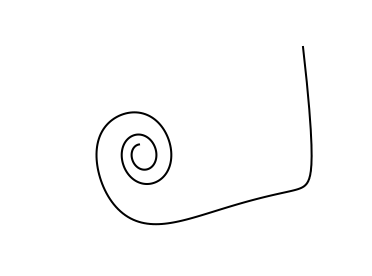
\includegraphics[scale=0.35]{figures/vanderpol-hopfbifurcation--0_1.png} \\ $\lambda = -0.1$ \\
	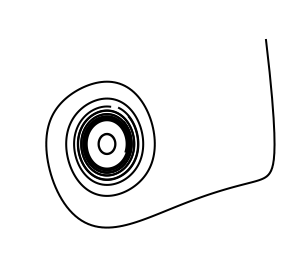
\includegraphics[scale=0.35]{figures/vanderpol-hopfbifurcation-0_0.png} \\ $\lambda = 0.0$ \\
	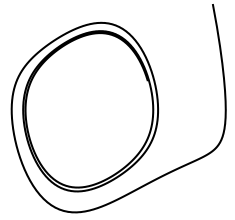
\includegraphics[scale=0.35]{figures/vanderpol-hopfbifurcation-0_1.png} \\ $\lambda = 0.1$ \\
	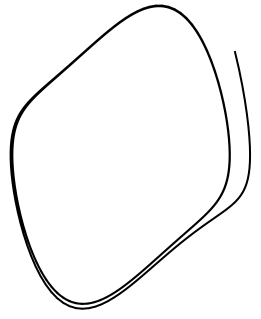
\includegraphics[scale=0.35]{figures/vanderpol-hopfbifurcation-0_3.png} \\ $\lambda = 0.3$
	\caption{$\clubsuit$ Bifurcación de Poincaré-Andronov-Hopf en el oscilador de Van der Pol.}
\end{figure}

\subsection{Bifurcación silla-nodo de ciclos}
En este tipo de bifurcación, relacionada con la bifurcación silla-nodo de puntos críticos (sección \ref{sec:bifurcacionsillanodo}), dos ciclos límite chocan y se anulan mutuamente.

El siguiente ejemplo ilustra la situación.

\begin{example} \label{ex:bifurcacionsillanododeciclos}
Considérese el sistema (en forma polar)

\begin{equation}
	\begin{array}{lll}
		\dot{r} & = & \lambda r + r^3 - r^5 \\
		\dot{\theta} & = & 1 + r^2
	\end{array}.
\end{equation}

Notemos primero que la ecuación $\dot{r} = \lambda r + r^3 - r^5$, considerada en sí misma como un sistema dinámico de una dimensión, sufre una bifurcación de silla-nodo cuando $\lambda = \bar{\lambda} = - \frac{1}{4}$. Este es el mismo valor de $\lambda$ crítico que consideraremos para el sistema bidimensional.

Vale la pena anotar que el sistema también sufre una bifurcación de Hopf cuando $\lambda = 0$ pero no es este el fenómeno de interés en este caso particular. Supondremos entonces que $\lambda < 0$ en todo momento y nos concentramos en el comportamiento alrededor del centro en $(0,0)$. Empezamos por notar que este punto crítico permanece estable y no participa en la bifurcación. 

\begin{itemize}
	\item Cuando $\lambda < \bar{\lambda}$ no hay órbitas cíclicas alrededor del origen.
	\item En $\lambda = \bar{\lambda}$, un ciclo límite semiestable aparece.
	\item Para $\lambda > \bar{\lambda}$ este ciclo se separa en otros dos ciclos límite: uno estable y otro inestable.
\end{itemize}

\begin{figure}[!ht] \centering
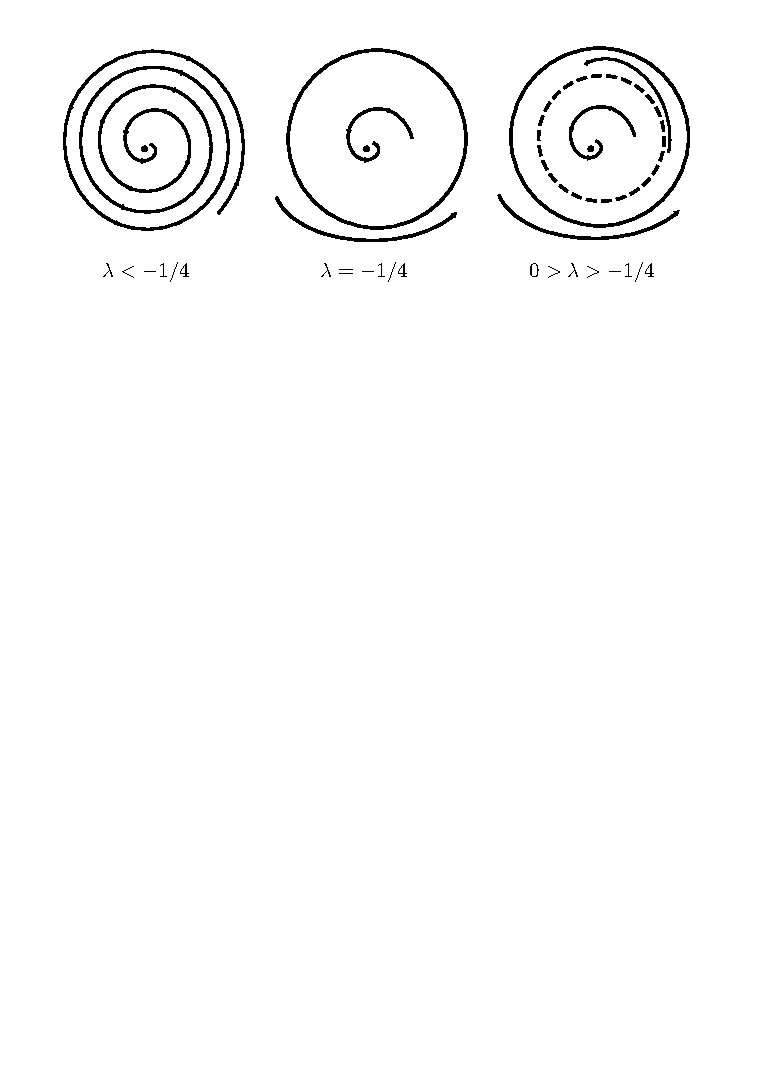
\includegraphics[scale=1.3]{figures/saddlenodecycles.pdf}
\label{fig:bifurcacionsillanododeciclos}
\end{figure}

\end{example}
